%! TEX root = ./main.tex

\lecture{08}{Week 4}{Implementing Dynamic Memory Allocation}


Sidenote: A Runtime allows a programming language to use C libraries. C does not have a runtime, therefore it is well suites for e.g. OS programming.

The OS allocates memory to the C program in pages. Using \verb+sbrk()+ we can request a new page from the OS. But we often only need a few bytes. A memory allocator is a interface which sits between the application and the memory and gives out memory blocks to applications. A block is a continuous range of bytes of any size.\\
\code{malloc} is such a dynamic memory allocator

\paragraph{Address Space}
The address space is split into multiple parts. The NULL pointer is at address $0x00000000$ and contains nothing. On top of it, at $0x00000008$ is the \textit{Text}. This section contains the machine code of our functions. On top of it is the \textit{Data} section, where global variables and parameters (?) are stored. On top of all that is the heap, which grows upwards. At the top, almost at $0xFFFFFFFF$, is the stack, which grown downwards. Functions of libraries, like \code{malloc} are dynamically linked and the address is determined at runtime. Addresses in the heap are not allocated linearly, but in some different fashion.

\paragraph{Explicit Memory Allocation}
Allocation and free is done manually by the user. All operations appear in the program source. After allocation, there is a point of time, from when on the object must be accessible. There is another point in time, before which the data object cannot be freed.

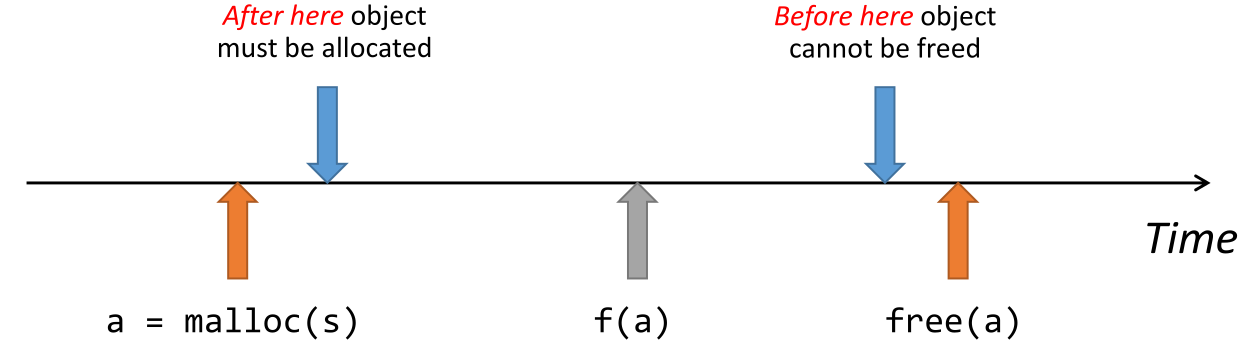
\includegraphics[width=0.8\textwidth]{08_memoryallocationcycle.png}

\paragraph{Implicit Memory Allocation}
The user allocates memory by creating new objects. But they are implicitly deallocated by a \textit{Garbage Collector}. After a new object is initialized, there is some point in time, where the allocation must be finished and the object must be available. There is again a point in time before which the object cannot be freed. Once the object becomes unreachable, meaning we do not habe a reference to the abject anymore (this does only work because such languages do not support pointers), the garbage collector frees the memory.

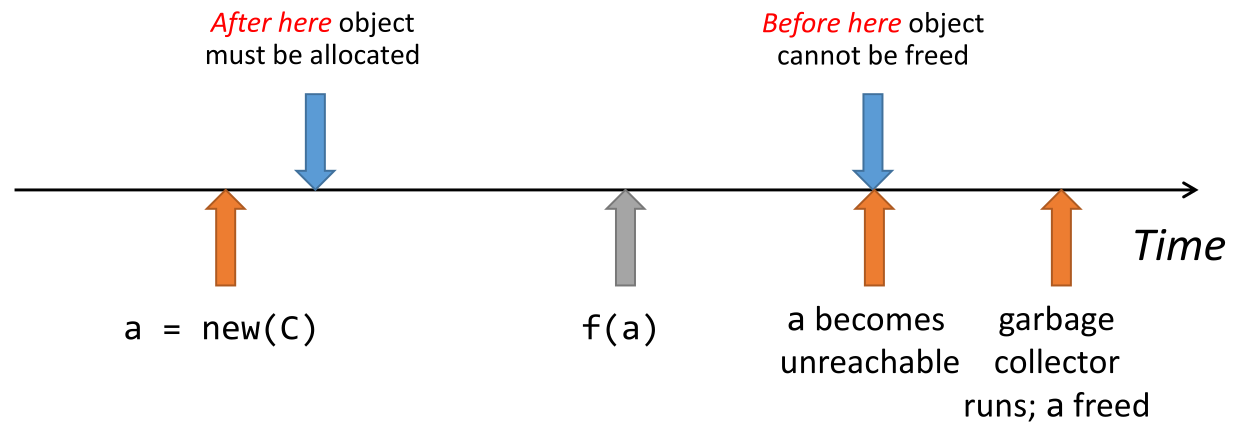
\includegraphics[width=0.8\textwidth]{08_garbagecollectedcycle.png}

\paragraph{Compiler Supported Memory Allocation}
The compiler proves from which point on a object must exist, and from which point on it is no longer required. This way the compiler decides when to allocate and deallocate occur. This makes a language extremely fast.

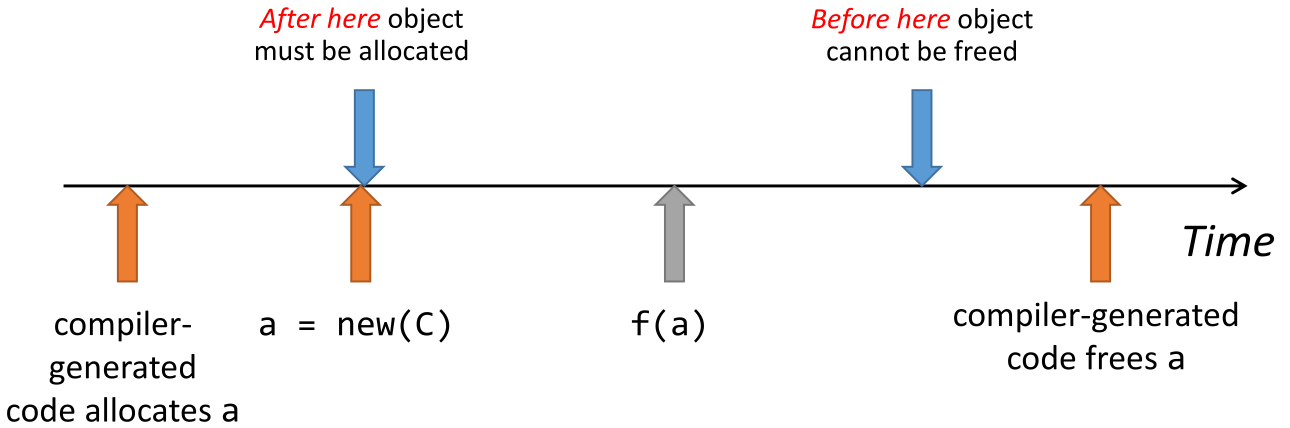
\includegraphics[width=0.8\textwidth]{08_compilersupportcycle.png}

All memory allocations use explicit allocation under the hood, therefore it is crucial to have a good understanding about it.

\subsubsection{The Problem}
In this lecture we assume that memory is word addressed. This has the advantage that each word can hold a pointer.

\paragraph{Constraints}
One of the difficulties is that in a program we can issue arbitrary sequences of allocate and deallocate. Memory allocators cannot control the number or size of allocated block and obviously they can only allocate free parts of the memory. Since they must respond immediately, they also have to time to reorder or buffer requests. Blocks must also be aligned to satisfy external requirements (8 byte alignment for GNU \code{malloc}). This means that the payload (/block) must always start at an alignment line (for better CPU performance). Once a block is allocated, this block cannot be moved or changes anymore.

\paragraph{Performance Goal}
Given a sequence of allocations and deallocations, we want to maximize the \textit{throughput} as well as the \textit{peak memory utilization}. These goals are conflicting by nature.

\subparagraph{Throughput}
The throughput is the number of requests per unit time. The goal is to perform allocations and deallocation operations in $O(1)$.

\subparagraph{Peak Memory Utilization}
The peak memory utilization defines how efficiently we use the available memory.

To measure the peak memory utilization we define for some sequence of allocations/deallocation $R_0, R_1 \dots R_k, \dots R_{n-1}$

\begin{description}
    \item[Aggregate playload $P_k$:] The sum of currently allocated payloads (the difference between all \code{malloc(p\_i)} and all \code{free(p\_j)}). Where a payload of $p$ bytes is generated by \code{malloc(p)}.
    \item[Current heap size $H_k$:] Assume $H_k$ is monotonically increasing.
    \item[Peak memory utilisation after $k$ requests $U_k$:] $(\text{max}_{i<k} P_i) / H_k$ 
\end{description}

\paragraph{Fragmentation}
Fragmentation may cause poor memory utilization. The two types of fragmentation are:

\begin{description}
    \item[Internal Fragmentation:] For a given block where the payload is smaller than the block size
        the payload is padded by unused unused space. Another cause is bookkeeping information, like start and end tags, are added.
    \item[External Fragmentation:] When there is enough free space on the heap, but not as a single free block.
\end{description}

While internal fragmentation is predictable and easy to measure, external fragmentation depends on the pattern of requests und therefore is difficult to predict and measure.

\paragraph{Size of a Memory Block}
In order that \code{free} knows how large the block of the memory to free is, \code{malloc} keeps track of the size of a memory block, by storing the size in the first word of the newly created memory block. The pointer it returns actually points on the second word.

\subsubsection{Keeping Track of Free Block}
The key policies for memory allocators are Placement policy (how do we find the block to use), Splitting policy (how do we split blocks which are too large) and Coalescing policy (how do we merge free blocks).

\paragraph{Implicit Free List}
For each block we need to know its size, as well as whether it is allocated or not. We store all these information in the first word of block. The allocated flag is actually the least signification bit of the length. This introduces some internal fragmentation (because the length up rounded up), but it can be neglected. Especial also since due to the alignment of block, some of the lower-order address bits are often anyways always $0$.

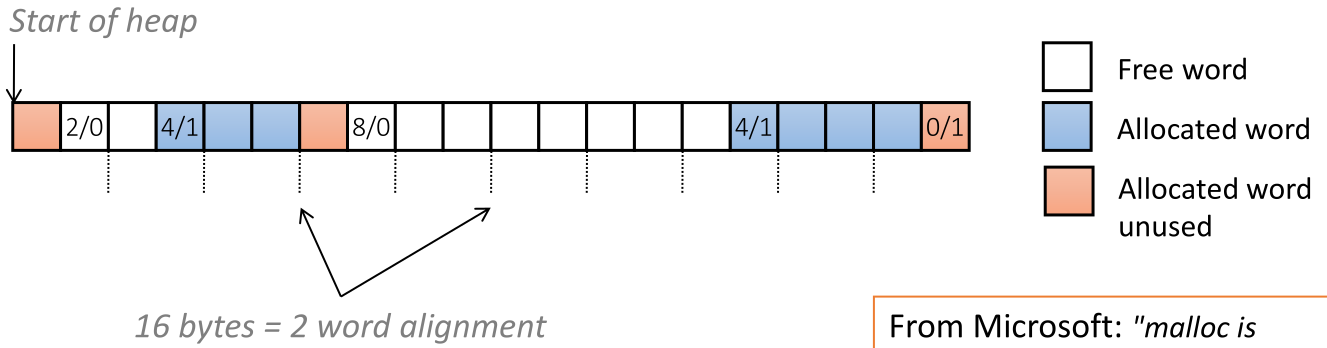
\includegraphics[width=0.8\textwidth]{08_implicit_free_list.png}

Due to alignment restrictions, the first word of the heap is never allocated.

\subparagraph{Finding a free block}
In order to find a free block, we iterate all blocks, starting from the first black, till we find the first free block which confirms to our space requirements. This approach takes linear time in the number of total blocks. In practice, we end up with many small blocks at the beginning of the list.

There are slight variations from this method:
\begin{description}
    \item[First Fit:] As described, takes the first suitable block from the beginning of the list
    \item[Next Fit:] As first fit, but does not start iteration from the beginning, but where it found a suitable free block the last time. This should be faster but may introduce more fragmentation.
    \item[Best Fit:] Iterates the whole list and takes the best fit (the one with the fewest bits left over). This keeps fragmentation small but is slower.
\end{description}

Often, we have to split an free block to not waste too much space.

\subparagraph{Freeing a block and coalescing}
When a block is freed, we do not want that a large free block is actually split in multiple small ones. Therefore, sequential free blocks should be merged into one large free block. This procedure is refereed to as \textit{coalescing}.\\
We can easily skip following free blocks by simple increasing the length of the freed block. This does logically ignore the length entry of the following free block.\\
In order to coalesce with previous block, we actually need to add an end tag/footer to each block, wich contains, equally as the header tag, the length of the block and a empty flag. This way we can coalesce previous blocks too by looking at the last word of the previous head.\\
Coalescing can be done in constant time for all possible allocated/unallocated scenarios.

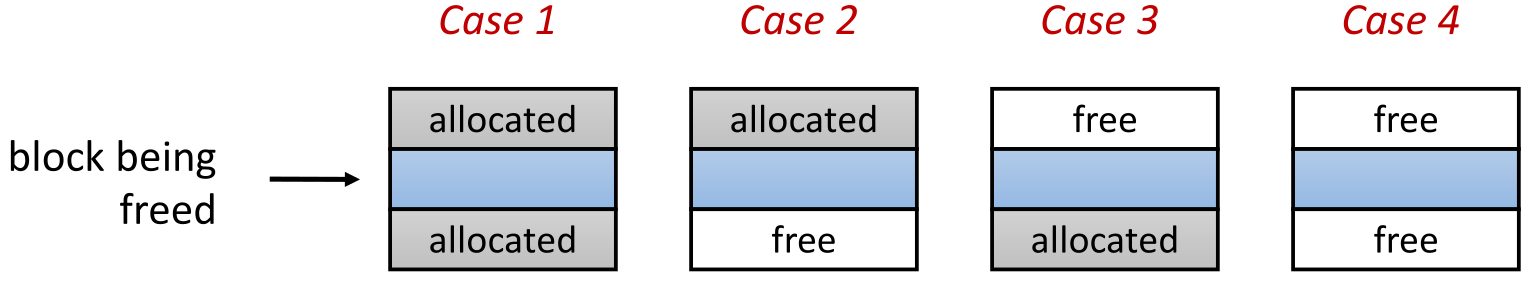
\includegraphics[width=0.8\textwidth]{08_coalecationsettings.png}

The additional end tag leads to internal fragmentation. 

\paragraph{Explicit free lists}
As the implicit list, it has an start tag and an end tag for coalescing. But in order to find free blocks, a pointer to the previous free block is stored in the first word of the payload area and in the second word, a pointer to the previous free block.

\subparagraph{Finding a free block}
We iterate our list and look for a valid block. In order to allocate a choose block we simple change the pointer pointing to our block.

\subparagraph{Freeing a block and coalescing}
In order to free a block simply add it to our list. There are multiple insertion policies which determine were in the list the new block is inserted:

\begin{description}
    \item[LIFO policy:] We insert the new block at the beginning of the list. This is simple to implement and has constant time. However, fragmentation may be worse.
    \item[Address-ordered policy:] We insert the blocks so that the address of the blocks are ordered. This requires search to find the desired location, but in turn, fragmentation should be better.
\end{description}

This method is faster than implicit free list, since the required time is linear in the number of free blocks.

\paragraph{Segregated free list}
Similar to the explicit free list. But in contrast to that, we keep separate lists blocks of different size. Most of the time, small blocks are allocated, hence this gives very good performance.

\subparagraph{Finding a free block}
To allocate a block of size $n$ we search the list of blocks of size $m > n$. On success, we split the block (if required) and place the fragment on the appropriate list. We do that on higher-level classes, till we have found a suitable block. If there is no such block, we request a new memory block from the OS. 

\subparagraph{Freeing a block and coalescing}
We coalesce the block and put in on the appropriate list.

The advantage of this method is the high throughput as well as the better memory utilisation.

Most allocated blocks are rather small. Segregated list give very good performance. Large blocks are only occasionally assigned. Many systems use this method.
